\section{Simulation Analysis}
\label{sec:simulation}

\par A simulation analysis was produced in order to better predict the behaviour of the circuit.

\par Starting with the obtained graphic for the output voltage in the gain stage as a function of time, we have:

\begin{figure}[h] \centering
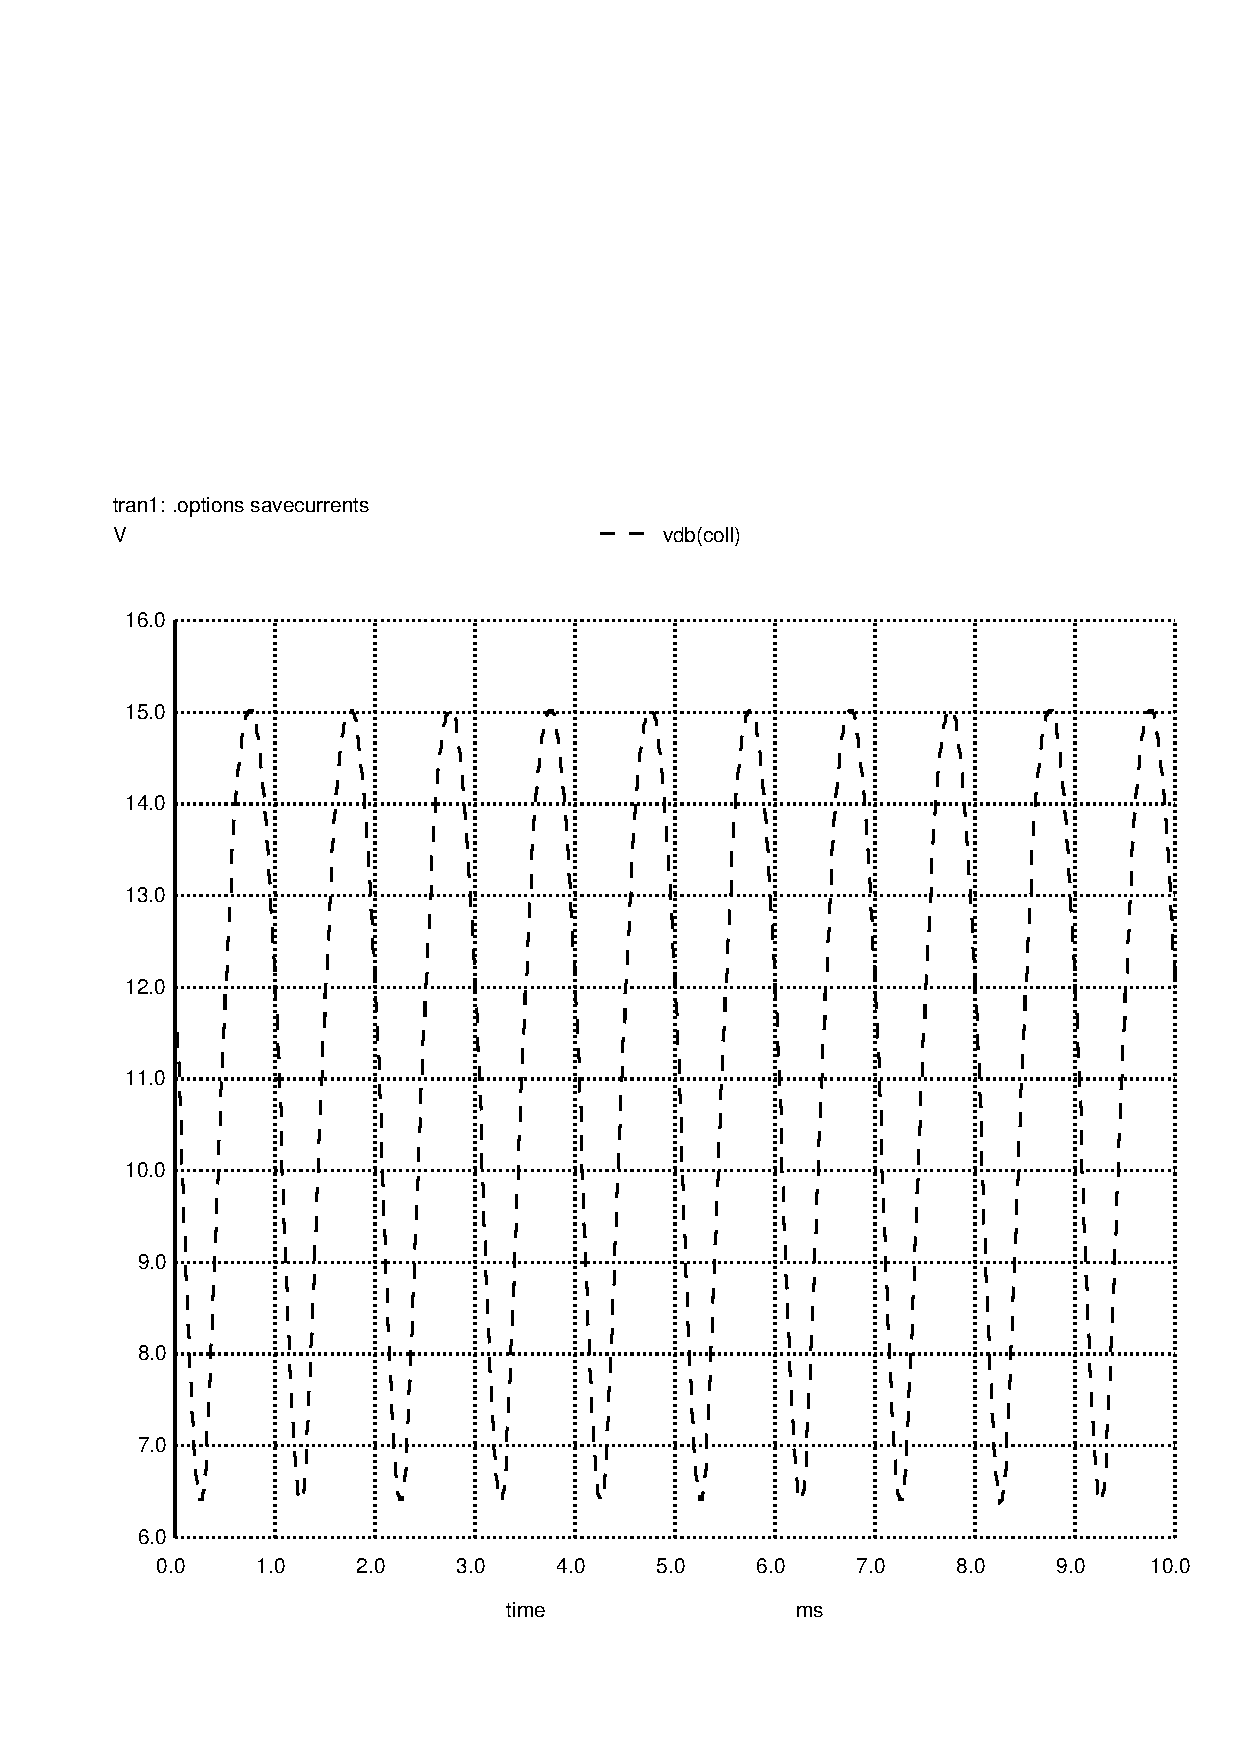
\includegraphics[width=0.6\linewidth]{../sim/vo1.pdf}
\caption{Output Voltage in the Gain Stage[v].}
\label{fig:vgain}
\end{figure}

\par One can see that there is no visible distortion on the sinusoidal signal.

\newpage

\par Figures \ref{fig:freqvg} and \ref{fig:freqvo} show the frequency response of the output voltage in the gain stage and output stage, respectively.


\begin{figure}[h] \centering
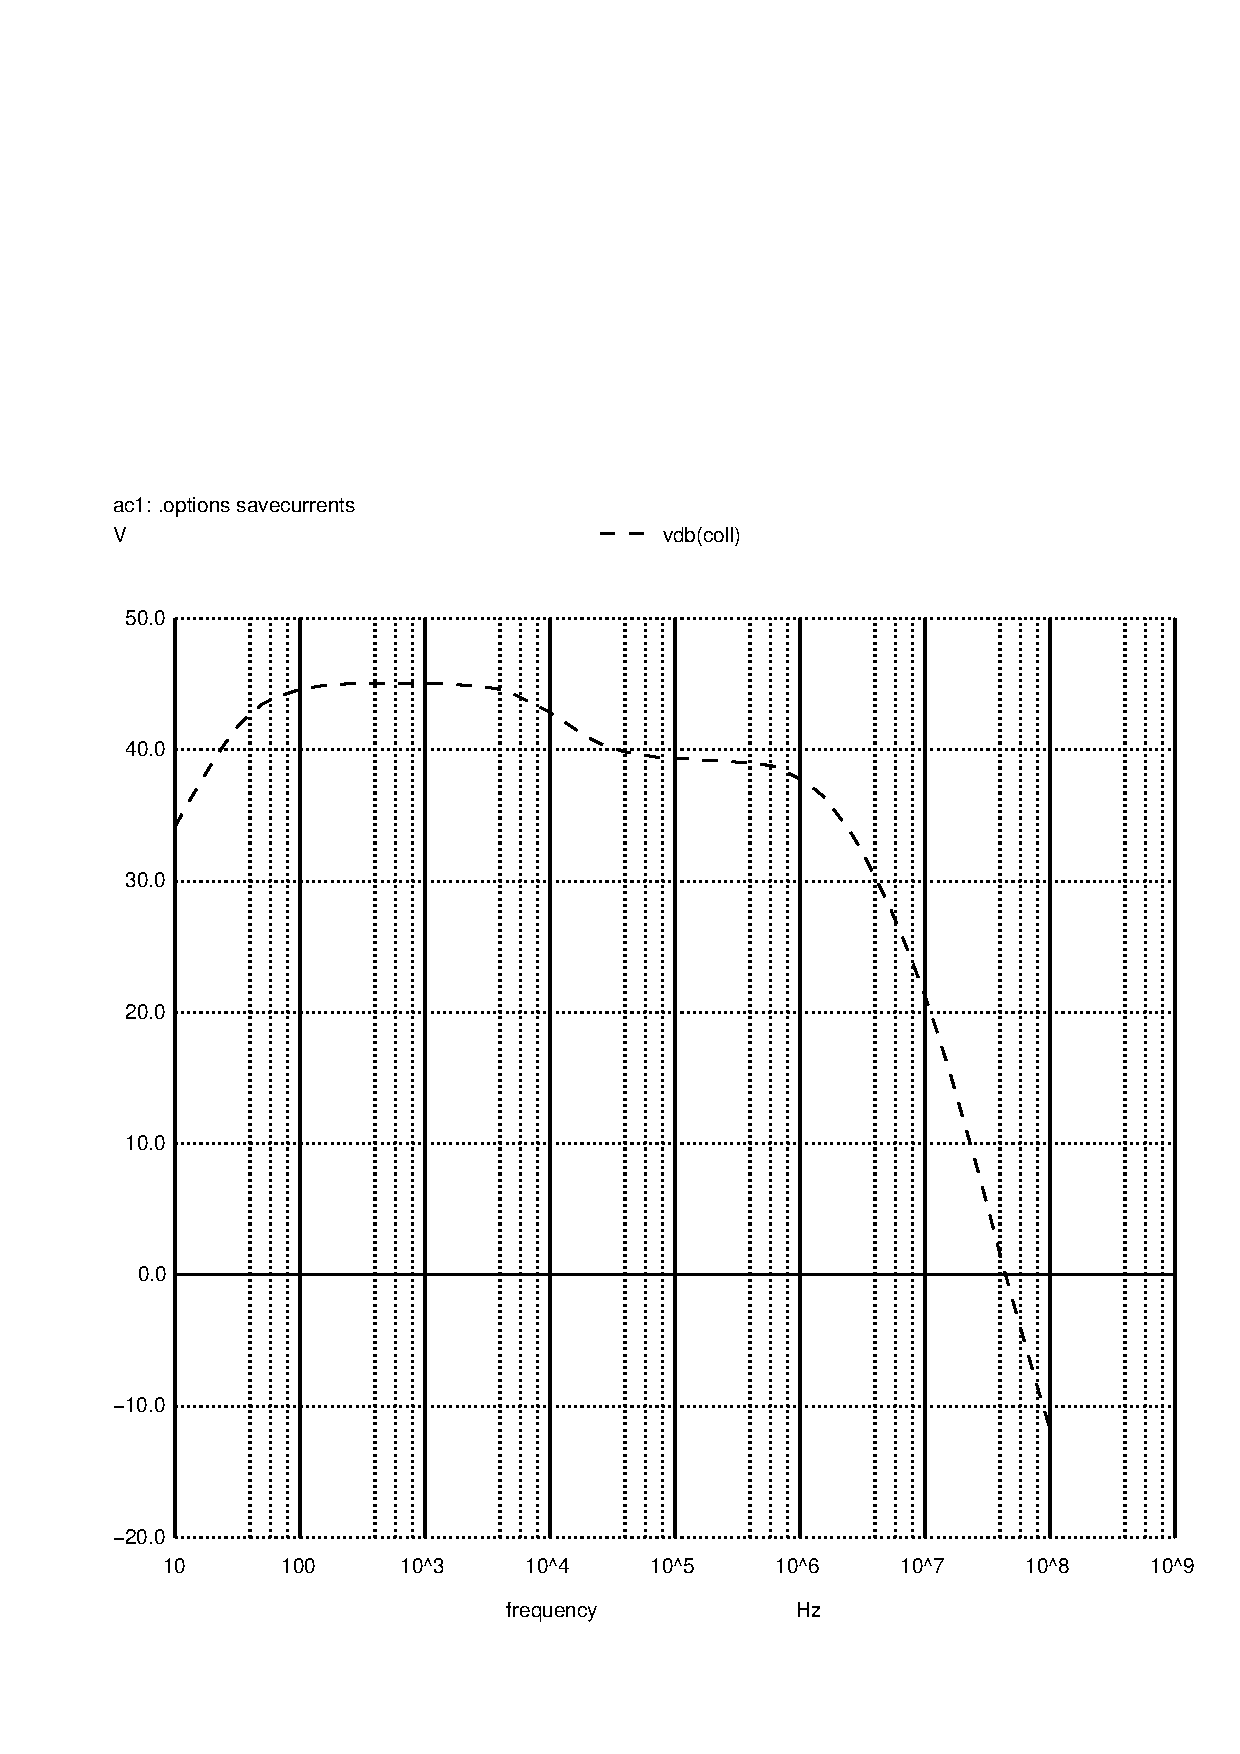
\includegraphics[width=0.6\linewidth]{../sim/vo1f.pdf}
\caption{Frequency response: Output Voltage in the Gain Stage..}
\label{fig:freqvg}
\end{figure}

\newpage

\begin{figure}[h] \centering
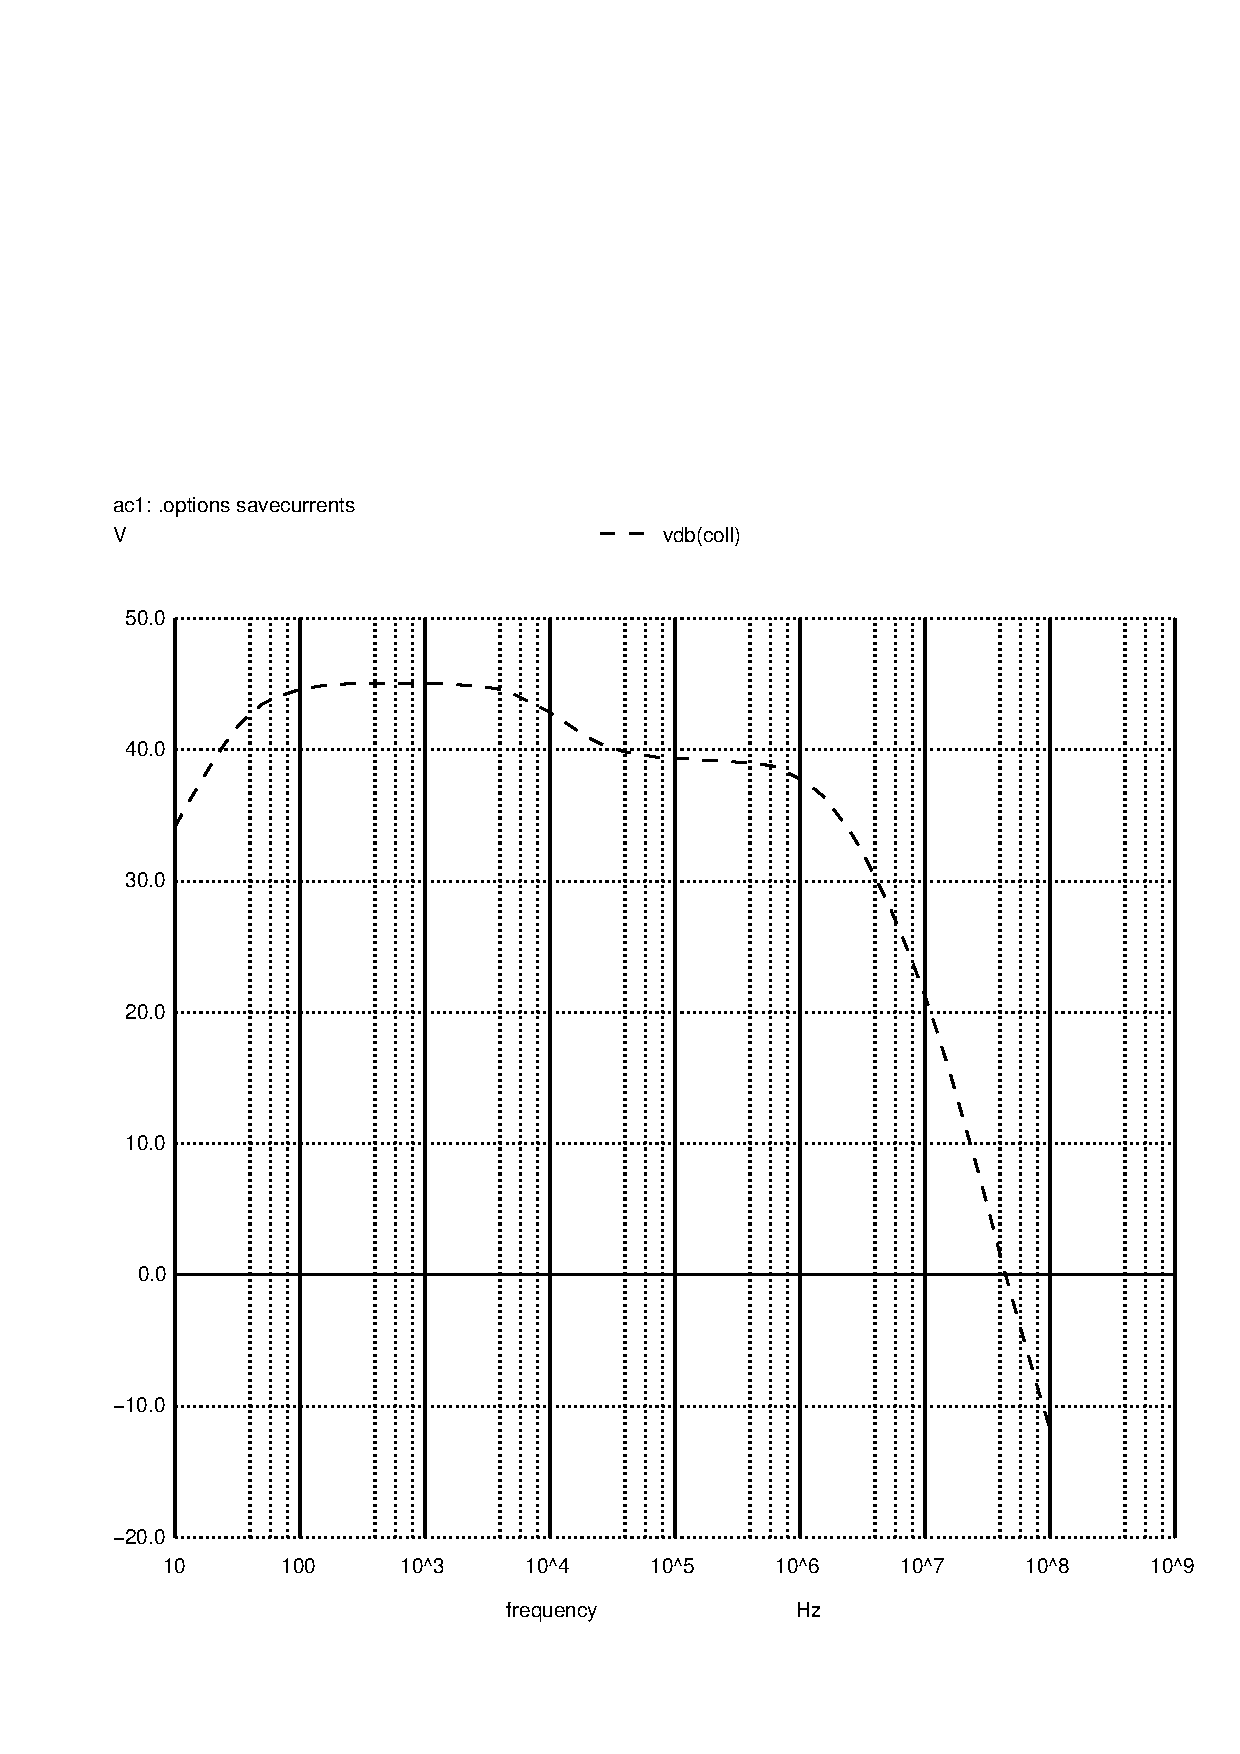
\includegraphics[width=0.6\linewidth]{../sim/vo2f.pdf}
\caption{Frequency response: Output Voltage in the Output Stage.}
\label{fig:freqvo}
\end{figure}

\newpage

\par The following graphic shows the frequency response of the gain produced by the circuit.

\begin{figure}[h] \centering
\includegraphics[width=0.6\linewidth]{../sim/gain.pdf}
\caption{Frequency response: Gain.}
\label{fig:freqgain}
\end{figure}

\newpage

\par Finally, the values for the most important quantities were simulated, resulting in the next tables:

\begin{table}[h]
  \centering
  \begin{tabular}{|l|r|}
    \hline    
   \input{../sim/Zin_tab}
   \end{tabular}
  \caption{Input Impedance.}
    \label{tab:zin}
\end{table}

\begin{table}[h]
  \centering
  \begin{tabular}{|l|r|}
    \hline    
    {\bf Name} & {\bf Value}\\ \hline
    \input{../sim/zout_tab}
  \end{tabular}
  \caption{Output Impedance.}
  \label{tab:zout}
\end{table}


\begin{table}[h]
  \centering
  \begin{tabular}{|l|r|}
    \hline    
    {\bf Name} & {\bf Value}\\ \hline
    \input{../sim/results_tab}
  \end{tabular}
  \caption{Simulated Results.}
  \label{tab:finalr}
\end{table}

\newpage

